\subsection{Modellbildung}
\label{subsec:02modellbildung}
Um eine Beziehung zwischen physikalischer Gr\"o\ss{}e f\"ur Geschwindigkeit und Lenkwinkel und der entsprechenden Stellgr\"o\ss{}e zu herzustellen, wird jeweils ein Modell ben\"otigt.
\paragraph{Geschwindigkeitsmodell} %TODO set math envirment
Die Daten aus Abbildung \ref{fig:velocity_profile} wurden bei einer Messfahrt mit Hilfe eines rosbag aufgezeichnet und im Anschluss mit dem Tool plotjuggler ausgewertet. Dazu wurde das Fahrzeug mit Geschwindigkeitsstellgr\"o\ss{}en im Intervall von -500 bis 1000 angesteuert und die jeweilige Geschwindigkeit aus der Odometrie ausgelesen. Auff\"allig ist der Sprung am Achsenursprung, der dadurch entsteht, dass das Fahrzeug eine bestimmte Stellgr\"o\ss{}e ben\"otig, um seine Tr\"agheit zu \"uberwinden.
Die gemessenen Daten lassen sich durch eine Gerade approximieren.

%%Akku
\begin{figure}[h] %TODO replace image
\centering
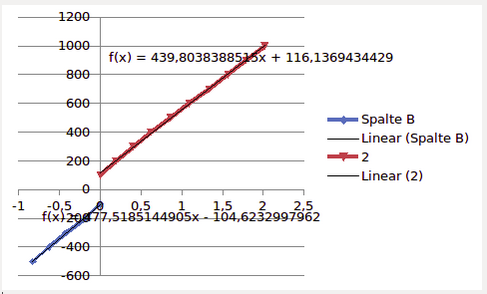
\includegraphics[width=0.7\linewidth]{pics/velocity_profile}
\caption{Geschwindigkeitsmodell}
\label{fig:velocity_profile}
\end{figure}

\paragraph{Lenkwinkelmodell}
Die Bestimmung des Lenkwinkelmodells (Abbildung \ref{fig:steering_profile}) folgte dem Schema:
\begin{itemize}
	\item Auto anheben und Stellgr\"o\ss{}e f\"ur den Lenkwinkel auf 0 setzen
	\item Mit Geschwindigkeit 300 kurz geradeaus fahren und dann Lenkwinkel einstellen
	\item Geschwindigkeit auf 0 setzen und den Lenkwinkel mit einem Geodreieck messen
\end{itemize}
Dazu war das Paket rqt\_reconfigure sehr hilfreich. Die gemessenen Daten wurden im Anschluss durch ein Polynome sechsten Grade approximiert. Auff\"alig ist die Verschiebung auf der y-Achse, die durch Offset in der Lenkung entsteht. Es sei angemerkt, dass die Messungen mit Fehlern behaftet waren und somit eine ungenaues Lenkwinkelmodell entstanden ist. Genauere Ergebnisse k\"onnte man mit Verwendung der Odometrie bei einer Fahrt im Kreis erzielen.
\begin{figure}[h] %TODO replace image
	\centering
	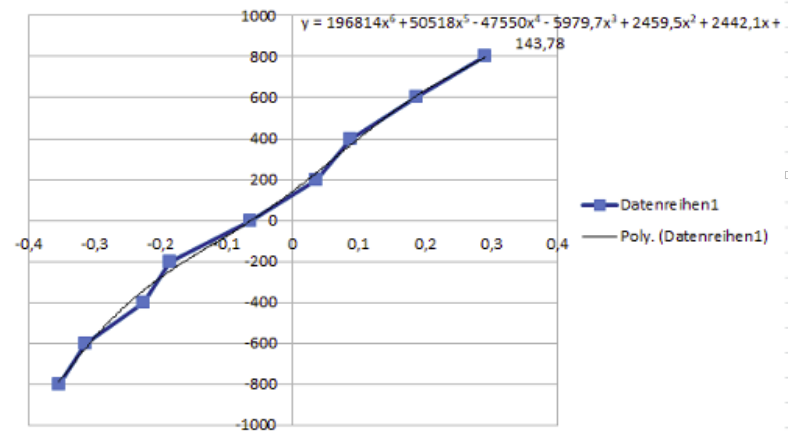
\includegraphics[width=0.7\linewidth]{pics/steering_profile}
	\caption{Lenkwinkelmodell}
	\label{fig:steering_profile}
\end{figure}